\section*{جواب سوال ۴}

\textbf{محاسبه امید ریاضی تعداد دفعاتی که باید تاس انداخته شود تا توالی عدد مضرب ۳ نباشد - عدد مضرب ۳ باشد - عدد مضرب ۳ نباشد مشاهده شود:}

برای حل این مسئله، ما از نظریه زنجیره‌های مارکوف استفاده می‌کنیم. سه حالت ممکن برای هر پرتاب تاس وجود دارد:

\begin{enumerate}
	\item حالت \(A\): هیچ عددی تاکنون پرتاب نشده یا آخرین عدد پرتاب شده مضرب ۳ نبوده است.
	\item حالت \(B\): آخرین عدد پرتاب شده مضرب ۳ بوده است.
	\item حالت \(C\): توالی کامل شده است (یعنی عدد مضرب ۳ نباشد - عدد مضرب ۳ باشد - عدد مضرب ۳ نباشد).
\end{enumerate}

ماتریس انتقال \(P\) به صورت زیر است:
\[ P = \begin{bmatrix}
	\frac{4}{6} & \frac{2}{6} & 0 \\
	\frac{1}{6} & 0 & \frac{5}{6} \\
	0 & 0 & 1
\end{bmatrix} \]

این ماتریس نشان‌دهنده احتمال جابه‌جایی بین حالت‌ها است.

برای محاسبه امید ریاضی تعداد دفعات پرتاب تاس تا رسیدن به حالت \(C\) بعد از حالت \(A\)، ما از خواص زنجیره‌های مارکوف استفاده می‌کنیم. این محاسبه شامل محاسبه زمان اولین ورود به حالت \(C\) از حالت \(A\) است.

در نمودار زنجیره مارکوف که برای مسئله داده شده رسم شده است، گره‌ها حالت‌های مختلف زنجیره را نشان می‌دهند و یال‌ها احتمال انتقال بین حالت‌ها را نمایش می‌دهند. 

\begin{itemize}
	\item حالت \(A\): این حالت نشان‌دهنده شروع توالی یا پرتاب عددی غیر مضرب ۳ است.
	\item حالت \(B\): این حالت نشان‌دهنده پرتاب عدد مضرب ۳ است.
	\item حالت \(C\): این حالت نشان‌دهنده اتمام توالی مورد نظر ما (عدد مضرب ۳ نباشد - عدد مضرب ۳ باشد - عدد مضرب ۳ نباشد) است.
\end{itemize}

\begin{figure}[H]
	\centering
	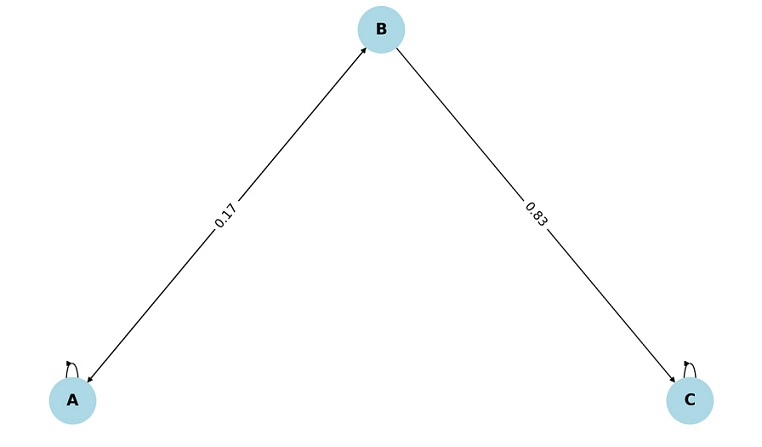
\includegraphics{pic2.jpg}
	\label{fig:label4}
\end{figure}